%%%%%%%%%%%%%%%%%%%%%%%%%%%%%%%%%%%%%%%%%
% Research Report Assignment Title Page 
% LaTeX Template
% Version 1.0 (06/03/16)
%
% This template has been downloaded from:
% http://www.LaTeXTemplates.com
%
% Original author: Francisco Maria Calisto
% WikiBooks (http://en.wikibooks.org/wiki/LaTeX/Title_Creation)
%
% License:
% CC BY-NC-SA 3.0 (http://creativecommons.org/licenses/by-nc-sa/3.0/)
% 
% Instructions for using this template:
% This title page is capable of being compiled as is. This is not useful for 
% including it in another document. To do this, you have two options: 
%
% 1) Copy/paste everything between \begin{document} and \end{document} 
% starting at \begin{titlepage} and paste this into another LaTeX file where you 
% want your title page.
% OR
% 2) Remove everything outside the \begin{titlepage} and \end{titlepage} and 
% move this file to the same directory as the LaTeX file you wish to add it to. 
% Then add \input{./title_page_1.tex} to your LaTeX file where you want your
% title page.
%
%%%%%%%%%%%%%%%%%%%%%%%%%%%%%%%%%%%%%%%%%
%\title{Title page with logo}
%------------------------------------------------------------------------------
%	PACKAGES AND OTHER DOCUMENT CONFIGURATIONS
%------------------------------------------------------------------------------

\documentclass[12pt]{article}
\usepackage[english]{babel}
\usepackage[utf8x]{inputenc}
\usepackage[T1]{fontenc}
\usepackage{amsmath}
\usepackage{graphicx}
\usepackage[colorinlistoftodos]{todonotes}
\usepackage{subcaption}
\usepackage{biblatex}
\usepackage{fontspec}

\addbibresource{bib.bib}

\begin{document}

\begin{titlepage}

\newcommand{\HRule}{\rule{\linewidth}{0.5mm}} % Defines a new command for the horizontal lines, change thickness here

\center % Center everything on the page
 
%------------------------------------------------------------------------------
%	HEADING SECTIONS
%------------------------------------------------------------------------------

% Name of your university/college
\textsc{\LARGE Instituto Superior T\'{e}cnico}\\[1.5cm]
% Major heading such as course name
\textsc{\Large ISR}\\[0.5cm]
% First Minor heading such as course title
\textsc{\large Report}\\[0.25cm]
% Second Minor heading such as course title
\textsc{\small State Of The Art Milestone}\\[0.25cm]

%------------------------------------------------------------------------------
%	TITLE SECTION
%------------------------------------------------------------------------------

\HRule \\[0.5cm]
{\large \bfseries Domain Questions and Observation}\\[0.25cm] % Title of your document
\HRule \\[0.5cm]
 
%------------------------------------------------------------------------------
%	AUTHOR SECTION
%------------------------------------------------------------------------------

\begin{minipage}{0.4\textwidth}
\begin{flushleft} \large
\emph{Author:}\\
Francisco Maria \textsc{Calisto} % Your name
\end{flushleft}
\end{minipage}
~
\begin{minipage}{0.4\textwidth}
\begin{flushright} \large
\emph{Coordinator:} \\
Jacinto \textsc{Nascimento} % Coordinator's Name
\end{flushright}
~
\begin{flushright} \large
\emph{Co-Coordinator:} \\
Daniel \textsc{Gon\c{c}alves} % Co-Coordinator's Name
\end{flushright}
\end{minipage}\\[2cm]

% If you don't want a supervisor, uncomment the two lines below and remove the section above
%\Large \emph{Author:}\\
%John \textsc{Smith}\\[3cm] % Your name

%-----------------------------------------------------------------------------
%	DATE SECTION
%-----------------------------------------------------------------------------

{\large 10/09/2016}\\[1cm] % Date, change the \today to a set date if you want to be precise

%-----------------------------------------------------------------------------
%	LOGO SECTION
%-----------------------------------------------------------------------------

% 
\includegraphics{ist-logo.png}\\[0.5cm] % Include a department/university logo - this will require the graphicx package

% 
\includegraphics{isr-logo.png}\\[0.5cm] % Include a department/university logo - this will require the graphicx package

\begin{figure}
\centering
\begin{subfigure}{.5\textwidth}
  \centering
  
\includegraphics[width=.5\linewidth]{isr-logo.png}
\end{subfigure}%
\begin{subfigure}{.5\textwidth}
  \centering
  
\includegraphics[width=.5\linewidth]{inesc-id-logo.png}
\end{subfigure}
\begin{subfigure}{.5\textwidth}
  \centering
  
\includegraphics[width=.25\linewidth]{ist-logo.png}
\end{subfigure}
\end{figure}
 
%-----------------------------------------------------------------------------

\vfill % Fill the rest of the page with whitespace

\end{titlepage}

\section{Introduction}

In the last meeting at the SAMS Hospital I brought with me two books, IRM du SEIN and Mammography Casebook, both recommended by Dr. Cristina da Fonseca that suggested a deep reading to a better understanding of the domain, its action field as precisely as IRM works in physical terms, but also the completed diagnosis. The second book contains 100 cases of complete breast cancer diagnosis. The latter provides all the information of clinical cases and prognosis thereof, thus allowing us, the researchers, to understand physicians difficulties on the clinical diagnosis.

\clearpage

\section{The Meetings}

On the 8st of September from 4 pm to 6 pm I meet Dr. Cristina da Fonseca at SAMS Hospital to give her their books and to make some questions about them.

The next day I meet Dr. Cristina da Fonseca in IMI at 11 am, as the first meeting at that location. Then I could observe how is the diagnosis and analysis of IMR and all laboratory dynamics, from devices to medical analysis, as well as the procedures of technicians.

\section{The Questions}

As usual reading information that is beyond our field produces interesting doubt where the answers are interesting both in understanding of the problem domain but also in understanding how to improve the interaction and the breast cancer diagnosis.

From the IRM du SEIN book I had my first question about what was {\it Saturation des Graisses} in english is called Fat Sat. The Fat Sat is a technique to remove the fat signal in IRM. This is a method that uses the slight difference in resonance frequency of protons of the hydrogen atoms present in fat compared to those of the water molecule. This difference is about 220 Hz (1.5 Tesla). Therefore sends a radio-frequency specifically directed to the frequency of the fat in order to saturate before collecting the cutting signal. The advantages of this method used in weighting as T1 and T2 is giving us a better highlight the contrast agent taken on T1. A new information appears here to us, the word T1 and T2, that the reading of the books was so important. In IRM physicians almost do two kinds of intensity with their own characteristics of diagnosis. It will be important since we will have more modalities of imaging inside IRM.

The second question was related to the Diffusion Coefficient where apparently  values are quantified by measurement of mean diffusivity along three orthogonal directions, which are affected by cellularity of the tissue, fluid viscosity, membrane permeability and blood flow.

An also important question about what are Mammography Artefacts since it is consider to be bugs into the image. This kind of information is important on the giving of less ambiguity of information and communication between researchers and physicians.

<----- TODO -----> analysis of an isolated enhancement MRI scheme

On Mammography Casebook it gave us a great overview of how classify and what to do in the different cases of the diagnosis, since this book has 100 cases of breast cancer diagnosis.

The first question we made about this boot was what is de Signal-to-time curve and what conclusion does this curve intend to interpret the percentage of maximal signal that will or not increase will tend to correlate very well to the density of the micro-vessel count. However this is important as a modalities of imaging diagnosis we will not implement this because is out of our focus requirements.

We also did not understood what was the word Specimen radiography means in terms of the clinical breast cancer domain but it was easy to understand with the simple and clear explanation of Dr. Cristina da Fonseca.



% Commands to include a figure:
%\begin{figure}[!hbt]
%\centering
%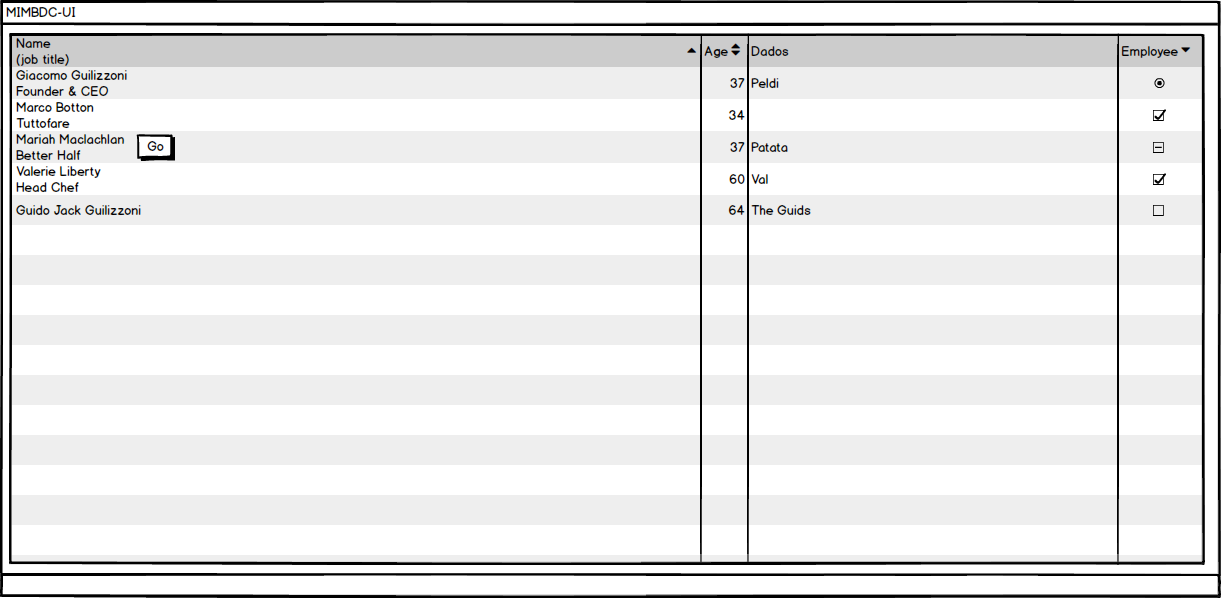
\includegraphics[width=1.00\textwidth]{tabela_pessoas.png}
%\caption{\label{PT}Table of People.
%}
%\end{figure}

\clearpage

\section{Conclusions}

\section{Acknowledgements}

This report will help our research project in cooperation between ISR \cite{isr} and INESC-ID \cite{inescid} both are associate institutes of Instituto Superior T\'{e}cnico \cite{ist}, Universidade de Lisboa \cite{ul}. Throughout this challenging journey we had the untiring and patient support from our family and friends.

We would like to give a special thanks to Dr. Cristina Ribeiro da Fonseca and Dr. Clara Aleluia who have cooperated with us tirelessly, thus making a major contribution to the national research and development of innovation in Portuguese clinical Information Systems.

We also want to thanks Bruno Cardoso, Rodrigo Louren\c{c}o, Bruno Oliveira, Tom\'{a}s Pinho, L\'{i}dia Freitas, Bruno Dias, Jo\~{a}o Miranda, Prof. Dr. Jacinto Nascimento, Prof. Dr. Daniel Gon\c{c}alves, Ana Beatriz Alves, Francisco Silveira, Joana Teixeira, Daniel Da Costa, Filipe Fernandes, In\^{e}s Fran\c{c}a Martins, Lu\'{i}s Ribeiro Gomes and Ricardo Cruz for helping, supporting and reviewing our work.

\clearpage

\printbibliography

\end{document}
